\documentclass[a4paper,12pt]{article}
\usepackage[utf8x]{inputenc}
\usepackage[swedish]{babel}
\usepackage[T1]{fontenc}
\usepackage{graphicx}
\usepackage{subcaption}
\usepackage{float}
\usepackage{placeins}
\usepackage{amsfonts, amsmath, amssymb}
\usepackage{ccfonts,euler}
\usepackage{wrapfig}
\usepackage{multirow}
\usepackage{caption}
\usepackage{enumerate}
\usepackage{comment}
\usepackage[includeheadfoot,margin=1.1in]{geometry}
\usepackage{hyperref}
\usepackage{listings}
\usepackage{color}

\definecolor{dkgreen}{rgb}{0,0.6,0}
\definecolor{gray}{rgb}{0.5,0.5,0.5}
\definecolor{mauve}{rgb}{0.58,0,0.82}

\lstset{frame=tb,
  language=Python,
  aboveskip=3mm,
  belowskip=3mm,
  showstringspaces=false,
  columns=flexible,
  basicstyle={\small\ttfamily},
  numbers=none,
  numberstyle=\tiny\color{gray},
  keywordstyle=\color{blue},
  commentstyle=\color{dkgreen},
  stringstyle=\color{mauve},
  escapeinside={\%*}{*)},
  breaklines=true,
  breakatwhitespace=true,
  tabsize=3,
  literate={å}{{\r a}}1 {ö}{{\"o}}1 {ä}{{\"a}}1 {Å}{{\r A}}1 {Ö}{{\"O}}1 {Ä}{{\"A}}1
}

\oddsidemargin -15mm
\evensidemargin -15mm
\marginparwidth 5mm
\topmargin -28mm
\textheight 282mm
\textwidth 190mm
\headheight 4mm
\headsep 4mm

\sloppy

\newcounter{iii}\setcounter{iii}{0}
\def\i{\bigskip\noindent\refstepcounter{iii}\textbf{\arabic{iii}.} }
%\def\iotst#1{\par \smallskip \mbox{}\refstepcounter{iii}\hspace*{#1}\textbf{\arabic{iii}.}}
\newcounter{pun}[iii]
\def\pu{\refstepcounter{pun}{\bf(\alph{pun})}\ }
\def\Pu{\par\noindent\mbox{}\refstepcounter{pun}{\phantom{\textbf{\arabic{iii}.}}\hspace{0.2mm}\bf(\alph{pun})}\ }

\def\ext{\subsection*{Extrauppgifter}}

\title{Programmering, Nao - Pass 6}
\date{3 augusti}

\makeatletter
\let\newtitle\@title
\let\newdate\@date
\makeatother
\begin{document}

  \renewcommand*\rmdefault{ppl}\normalfont\upshape
\pagestyle{empty}
\large
\section*{\newdate\ \  \newtitle}

\i \textbf{Permutationer}

\pu Skriv ett program som skriver ut alla möjliga strängar, av längd 3, som man kan bilda med bokstäverna  'a', 'b' och 'c'. Det ska bli 27st strängar, varför? 

\pu Modifiera programmet i a) så att varje bokstav bara får förekomma en gång. Det ska bli 6st strängar, varför?

\pu Skriv ut alla permutationer av strängen ''PEDRO''. 



\i \textbf{Send more money}

Ersätt varje bokstav med en unik siffra mellan 0 och 9 så att uträkningen i figur~\ref{sendmoremoney} stämmer. Notera att talen inte kan börja med 0, för i så fall skulle man kunna strunta i att skriva ut första bokstaven. 

\begin{figure}[!ht]
\centering
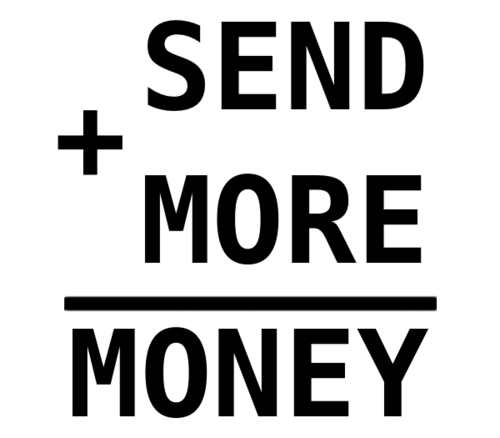
\includegraphics[width=0.3\textwidth]{sendmoremoney}
\caption{}
\label{sendmoremoney}
\end{figure}

\begin{comment}
tal = ['0', '1', '2', '3', '4', '5', '6', '7', '8', '9']
for s in tal[1:]:
    tal_e = tal[:]
    del tal_e[tal_e.index(s)]
    for e in tal_e[:]:
        tal_n = tal_e[:]
        del tal_n[tal_n.index(e)]
        for n in tal_n[:]:
            tal_d = tal_n[:]
            del tal_d[tal_d.index(n)]
            for d in tal_d[:]:
                tal_m = tal_d[:]
                del tal_m[tal_m.index(d)]
                for m in tal_m[:]:
                    if m != '0':
                        tal_o = tal_m[:]
                        del tal_o[tal_o.index(m)]
                        for o in tal_o[:]:
                            tal_r = tal_o[:]
                            del tal_r[tal_r.index(o)]
                            for r in tal_r[:]:
                                tal_y = tal_r[:]
                                del tal_y[tal_y.index(r)]
                                for y in tal_y[:]:
                                    send = int(s+e+n+d)
                                    more = int(m+o+r+e)
                                    money = int(m+o+n+e+y)
                                    if (send + more) == money:
                                        print('s = ', s, ', e = ', e, ', n = ', n, ', d = ', d, ', m = ', m, ', o = ', o, ', r = ', r, ', y = ', y)
                                        print("send = ", send, " more = ", more, ", money = ", money)
\end{comment}

\i \textbf{Lagomvinklade trianglar}

En lagomvinklad triangel är vad vi i denna uppgift kallar en triangel där minst en av vinklarna är exakt 60 grader. De lagomvinklade trianglarna känner sig ofta förbisedda jämfört med de mycket mer kända rätvinkliga trianglarna (så kallat mindervinkelkomplex), trots att de lagomvinklade också har en snygg formel för sina sidlängder:

${\displaystyle c^{2}=a^{2}+b^{2}-ab}$

Skriv ett program som skipar lite rättvisa i detta triangeldrama genom att fråga efter ett tal N (mellan 1 och 100) och sedan skriva ut hur många lagomvinklade trianglar det finns vars sidor är heltal i intervallet 1 till N.


\begin{figure}[!ht]
\centering
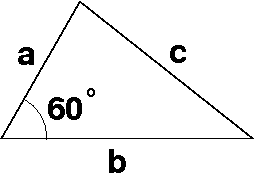
\includegraphics[width=0.3\textwidth]{triangel}
\caption{Ett exempel på en lagomvinklad triangel med sidlängderna $a = 5, b = 8$ och $c = 7$.}
\label{triangel}
\end{figure}
\newpage
\textbf{Körningsexempel}
\begin{lstlisting}
Talet N ? 25 
Antal trianglar: 35

Talet N ? 70
Antal trianglar: 112
\end{lstlisting}

\begin{comment}
N = int(input("N = "))
antal_trianglar = 0
for a in range(1,N+1): # Testar alla tal 1 till N för a
    for b in range(1,N+1): # Testar alla tal 1 till N för b
        for c in range(1,N+1): # Testar alla tal 1 till N för c
            if (c**2) == (a**2 + b**2 - a*b): # testar att formeln stämmer
                antal_trianglar += 1 #lägger då till en triangel
"""
Antalet trianglar som är beräknade 2 gånger
(spegelvända, a->b, b->a) = antal_trianglar-N
Eftersom det finns N stycken trianglar som är liksidiga,
resten ger dubbletter. Måste därefter addera N igen:
"""
print("antal trianglar: ", int((antal_trianglar-N)/2 + N))

\end{comment}

\i \textbf{Klockan}


\begin{figure}[!ht]
\centering
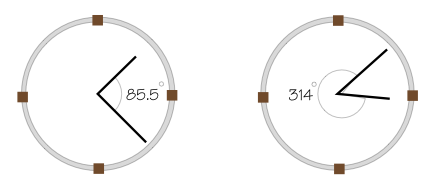
\includegraphics[width=0.5\textwidth]{klocka}
\caption{}
\label{fig:klocka}
\end{figure}

Om någon frågar hur mycket klockan är, svarar de flesta ''kvart över fem'', 15:29 eller något liknande. Vill man göra det lite svårare så kan man annars svara med vinkeln mellan tim- och minutvisaren, eftersom man ur denna information entydigt kan bestämma klockslaget. Dock är det många människor som är ovana vid detta sätt att ange tider, så det vore bra att ha ett datorprogram som översätter till ett mer normalt format. Du ska skriva ett sådant program.

Vi förutsätter att vår klocka saknar sekundvisare och endast visar ett helt antal minuter (det vill säga: båda visarna hoppar framåt bara på hel minut). Vinkeln avläses genom att utgå från timvisaren och sedan mäta hur många grader medurs minutvisaren ligger (se figur \ref{fig:klocka}). För att undvika decimaler anges vinkeln i tiondels grader (så att 85.5 grader skrivs som 855). Detta tal är alltid ett heltal mellan 0 och 3595 (inklusive) och är, som en följd av att endast hela minuter visas, alltid delbart med 5.

Programmet ska fråga efter en vinkel och sedan skriva ut tiden i vanligt digitalformat, alltså h:mm eller hh:mm, beroende på antalet timmar. Vi förutsätter att det är morgon, så alla tider ska ligga mellan 0:00 och 11:59 (inklusive).

\textbf{Två körningsexempel}
\begin{lstlisting}
Vinkel ? 855 
Klockan är 1:21

Vinkel ? 3140  
Klockan är 3:08
\end{lstlisting}

\begin{comment}
vinkel = int(input("Vinkel = "))

vinkel_timme = 0 #startar med 0 grader vid 00:00
for timme in range(12): #För alla timmar på förmiddagen
    vinkel_minut = 0 #startar med 0 grader vid varje hel timme
    for minut in range(60): #För alla minuter
        if vinkel_minut>vinkel_timme: #kollar om vi får en positiv vinkelskillnad från timmvisare till minutvisare
            if (vinkel_minut-vinkel_timme) == vinkel: #om vinkelskillnaden är lika med den önskade vinkeln
                if minut < 10: #för fin utskrift kollar vi storleken på minuter
                    print(str(timme)+":0" +str(minut)) #lägger till en nolla före minutrarna ifall vi har ett ental
                else:
                    print(str(timme)+":"+str(minut)) #annars skrivs det ut som det är
        else:
            if 3600-(vinkel_timme-vinkel_minut) == vinkel: #om vinkelskillnaden är negativ lägger vi till 360 grader
                if minut < 10:
                    print(str(timme)+":0" +str(minut))
                else:
                    print(str(timme)+":"+str(minut))
        vinkel_timme += 5 #360 grader/60 minuter/12 timmar, 1 min på timmvisaren = 0.5 grader
        vinkel_minut += 60 #360 grader/60 minuter, 1 min på minutvisaren = 6 grader
\end{comment}

\newpage

\i \textbf{Busig dotter}

En bonde har fem höbalar. Han bad sin dotter som deltagit på mattekollo att väga upp balarna åt honom, men istället för att väga dem en och en, valde hon att väga dem i parvisa kombinationer: bal 1 och 2, bal 1 och 3, bal 1 och 4, bal 1 och 5, bal 2 och 3, bal 2 och 4, osv. 

Vikterna för dessa parvisa vägningar skrev hon upp på 10 papperslappar. Men sen glömde hon bort vilken lapp som hörde till vilket par så hon tänkte ''Äsch, det spelar ju ingen roll, jag lägger dem i storleksordning.''

Nu står bonden här och har ingen aning om vilken höbal som väger vad. Det enda han har är papperslapparna. Kan du  hjälpa honom att reda ut det här? Hur mycket väger varje höbal? Finns det fler en än lösning? 

\textbf{Körningsexempel}
\begin{lstlisting}
Papperslappar ?  80, 82, 83, 84, 85, 86, 87, 88, 90, 91
Höbalarna väger: 39 41 43 44 47
\end{lstlisting}


\begin{comment}
rad = input("Papperslappar ? ").split(" ")
answers = [int(e) for e in rad]#[80, 82, 83, 84, 85, 86, 87, 88, 90, 91]

for a in range(50):
    for b in range(a,50):
        for c in range(b,50):
            for d in range(c,50):
                for e in range(d,50):
                    if sorted([a+b, a+c, a+d, a+e, b+c, b+d, b+e, c+d, c+e, d+e]) == answers:
                        print(a,b,c,d,e)
\end{comment}




\i \textbf{Tvetydiga datum}

Datum skrivs på olika sätt i olika länder. Till exempel skulle datumet 03/05/01 i Sverige betyda 1 maj 2003, medan det i USA skulle vara 5 mars 2001 och i en del andra länder 3 maj 2001 (vi kan utgå ifrån att årtalet alltid är under 2000-talet, dvs mellan 2000 och 2099).

Detta kan bland annat orsaka bekymmer när man tittar på bäst-före datumet på en gammal konservburk. Om man inte har en aning om vilket format ett datum har, kan man behöva pröva alla möjligha betydelser och, för att vara på den säkra sidan, välja det tidigaste giltiga datumet.

För att ett datum ska vara giltigt måste förstås månaden vara mellan 1 och 12 och dagen mellan 1 och antalet dagar i månaden. Antalet dagar i de tolv månaderna är i tur och ordning

31, 28, 31, 30, 31, 30, 31, 31, 30, 31, 30, 31

utom under skottår (vilka, för perioden 2000 − 2099, infaller om årtalet är jämnt delbart med 4) då februari har 29 dagar.

Skriv ett program som läser in de tre delarna av ett datum och skriver ut det tidigaste giltiga datumet som indata kan tänkas representera.

\textbf{Körningsexempel}
\begin{lstlisting}
Del 1: 3
Del 2: 5
Del 3: 1
År 2001, månad 3, dag 5.
\end{lstlisting}

\begin{comment}
from datetime import date

a = int(input("Del 1: "))
b = int(input("Del 2: "))
c = int(input("Del 3: "))

datum = []
try:
    datum.append(date(2000+a,b,c))
except:
    pass
try:
    datum.append(date(2000+a,c,b))
except:
    pass
try:
    datum.append(date(2000+b,a,c))
except:
    pass
try:
    datum.append(date(2000+b,c,a))
except:
    pass
try:
    datum.append(date(2000+c,a,b))
except:
    pass
try:
    datum.append(date(2000+c,b,a))
except:
    pass

minsta = min(datum)
print("Year: "+ str(minsta.year) + ", Month: " + str(minsta.month) + ", Day: " + str(minsta.day))
\end{comment}



\i \textbf{Uppställning}


\begin{figure}[!ht]
\centering

\includegraphics[width=0.35\textwidth]{uppstallning}
\caption{Raden med barn i exemplet sedda bakifrån.}
\label{uppstallning}
\end{figure}

En grupp med 8 barn, låt oss kalla dem A, B, C upp till H, beslutar sig för att testa din tankeförmåga. Utan att du ser dem ställer de upp sig på en rad. Sen räknar vart och en av dem hur många av de barn som står till vänster om honom/henne som är längre än han/hon själv, och sedan likadant med dem som står till höger. Var och en skriver ner dessa antal på en lapp som de ger till dig efter att ha frångått uppställningen. Deras enkla uppmaning till dig är att tala om i vilken ordning de stod.

Ett exempel med fem barn visas i figur \ref{uppstallning} ovan. A har ett längre barn (D) till vänster om sig och två (C och E) till höger. B har tre längre barn till vänster om sig och ett till höger. C har ett längre barn till vänster om sig men inget till höger och så vidare. Informationen på lapparna kan sammanfattas så här:

\begin{center}
  \begin{tabular}{ c | c | c }
Barn& Vänster & Höger \\ \hline
A	& 1 	  & 2     \\
B	& 3 	  & 1     \\
C	& 1 	  & 0     \\
D	& 0 	  & 0     \\
E	& 2 	  & 0     \\
  \end{tabular}
\end{center}

Tyvärr klarade du inte nöten utan måste i hemlighet smyga iväg och skriva ett datorprogram som löser uppgiften. Du kan förutsätta att alla barn är olika långa och att de inte har gjort något misstag när de skrev lapparna. Intressant nog finns det aldrig mer än en lösning. 


\textbf{Körningsexempel}
\begin{lstlisting}
Barn A, vänster ? 2
Barn A, höger ?  0
Barn B, vänster ? 0
Barn B, höger ? 1
Barn C, vänster ? 0
Barn C, höger ? 6
Barn D, vänster ? 2
Barn D, höger ? 3
Barn E, vänster ? 0
Barn E, höger ? 0
Barn F, vänster ? 3
Barn F, höger ? 1
Barn G, vänster ? 2
Barn G, höger ? 1
Barn H, vänster ? 6
Barn H, höger ? 1

Uppställningen: C B E D G F H A 
\end{lstlisting}

\begin{comment}
"""
#----- Exempel -----
# person = [antal högre personer till vänster, antal högre personer till höger]
A = [1,2]
B = [3,1]
C = [1,0]
D = [0,0]
E = [2,0]
personer = {'A':A, 'B':B, 'C':C, 'D':D, 'E':E}
#Ger uppställningen: D A C B E
"""
A = [2,0]
B = [0,1]
C = [0,6]
D = [2,3]
E = [0,0]
F = [3,1]
G = [2,1]
H = [6,1]
personer = {'A':A, 'B':B, 'C':C, 'D':D, 'E':E, 'F':F, 'G':G, 'H':H}

langdordning = [] #längdorning, längst till kortast
uppstallning = [] #ordningen dom står i
for i in range(len(personer)):
    langdordning.append("") #skapar tomma listor med samma längd som antalet personer
    uppstallning.append("")

for person in personer: #jämför längden på personerna och lägger till dom i storleksordning
    antal_langre_personer = personer[person][0] + personer[person][1]
    langdordning[antal_langre_personer] = person

for person in langdordning: #kollar personerna i längdordning och placerar dom på rätt plats
    antal_personer_till_vanster = personer[person][0] #antal personer till vänster
    #flyttar personerna som ska ligga till höger om personen ett steg till höger, och gör plats för personen vi ser på:
    uppstallning[antal_personer_till_vanster+1:] = uppstallning[antal_personer_till_vanster:-1]
    uppstallning[antal_personer_till_vanster] = person #personen tar samma index som antalet personer till vänster
    
print("uppställning: ", uppstallning)
\end{comment}

\end{document}
